%%%%%%%%%%%%%%%%%%%%%%%%%%%%%%%%%%%%%%%%
%% MCM/ICM LaTeX Template %%
%% 2025 MCM/ICM           %%
%%%%%%%%%%%%%%%%%%%%%%%%%%%%%%%%%%%%%%%%
\documentclass[12pt]{article}
\usepackage{geometry}
\geometry{left=1in,right=0.75in,top=1in,bottom=1in}

%%%%%%%%%%%%%%%%%%%%%%%%%%%%%%%%%%%%%%%%
% Replace ABCDEF in the next line with your chosen problem
% and replace 1111111 with your Team Control Number
\newcommand{\Problem}{Problem C Trading}
\newcommand{\Team}{Ahad Jiva}
%%%%%%%%%%%%%%%%%%%%%%%%%%%%%%%%%%%%%%%%

\usepackage{newtxtext}
\usepackage{amsmath,amssymb,amsthm}
\usepackage{newtxmath} % must come after amsXXX

\usepackage[pdftex]{graphicx}
\usepackage{lastpage}
\usepackage{xcolor}
\usepackage{fancyhdr}
\usepackage{listings}
\usepackage{xcolor}

\definecolor{codegreen}{rgb}{0,0.6,0}
\definecolor{codegray}{rgb}{0.5,0.5,0.5}
\definecolor{codepurple}{rgb}{0.58,0,0.82}


\lstdefinestyle{mystyle}{
    numberstyle=\tiny\color{codegray},
    basicstyle=\ttfamily\footnotesize,
    breakatwhitespace=false,         
    breaklines=true,                 
    captionpos=b,                    
    keepspaces=true,                 
    numbers=left,                    
    numbersep=5pt,                  
    showspaces=false,                
    showstringspaces=false,
    showtabs=false,                  
    tabsize=2
}

\lstset{style=mystyle}
\lhead{Team \Team}
\rhead{}
\cfoot{}

\newtheorem{theorem}{Theorem}
\newtheorem{corollary}[theorem]{Corollary}
\newtheorem{lemma}[theorem]{Lemma}
\newtheorem{definition}{Definition}

%%%%%%%%%%%%%%%%%%%%%%%%%%%%%%%%
\begin{document}
\graphicspath{{/figures}}  % Place your graphic files in the same directory as your main document
\DeclareGraphicsExtensions{.pdf, .jpg, .tif, .png}
\thispagestyle{empty}
\vspace*{-16ex}
\centerline{\begin{tabular}{*3{c}}
	\parbox[t]{0.3\linewidth}{\begin{center}\textbf{Problem Chosen}\\ \Large \textcolor{red}{\Problem}\end{center}}
	& \parbox[t]{0.3\linewidth}{\begin{center}\textbf{2024\\ MCM/ICM\\ Summary Sheet}\end{center}}
	& \parbox[t]{0.3\linewidth}{\begin{center}\textbf{Team Control Number}\\ \Large \textcolor{red}{\Team}\end{center}}	\\
	\hline
\end{tabular}}
\setlength{\parskip}{16pt} 
%%%%%%%%%%% Begin Summary %%%%%%%%%%%
% Enter your summary here replacing the (red) text
% Replace the text from here ...
\begin{center}
    \Large
    \textbf{Summary} \\
\end{center}

    In recent times, bitcoin has seen an almost incomprehensible surge in valuation surpassing the growth of virtually every conventional investment asset by a huge margin.
    This makes bitcoin an attractive asset for investors and traders who are open to riskier assets that may not have the slow but consistent growth of conventional financial instruments.
    In this problem, our goal is to use a mathematical model to take advantage of this growth to generate profits. We will also be trading gold, a conventional asset whose growth is not nearly
    as explosive but much more consistent and stable.
    Five years of price data for bitcoin and gold is given. With this data, the goal is to develop a mathematical model that makes optimal daily trades using only previous price data. 
    \$1000 is given at the start, and the model must make as much profit as possible.
    This solution uses mean reversion, the idea that asset prices in the long run will revert to their averages. Using the five years of price data given, a moving average is tracked as time passes
    and the model will either buy if the price is below the average (indicating potential future upside) or sell if above the average (indicating potential decline). The main parameter being modified
    is the window size of the moving average, i.e. how many days in the past the model is looking to calculate the moving average from which it makes its trading decisions.

    Our model uses this strategy across a range of moving average window sizes, from just one day to 250 days. The goal is to find the optimal window size that results in the most valuable portfolio
    at the end of the five year period. Further, our implementation of the model in Python allows for quick adjustments to other parameters like trade commissions. We will explore how these parameters affect
    final portfolio value and identify the optimal trading strategy.


    
% to here
%%%%%%%%%%% End Summary %%%%%%%%%%%

%%%%%%%%%%%%%%%%%%%%%%%%%%%%%%
\clearpage
\pagestyle{fancy}
% Uncomment the next line to generate a Table of Contents
\tableofcontents
\newpage
\setcounter{page}{1}
\rhead{Page \thepage\ of \pageref{LastPage}}
%%%%%%%%%%%%%%%%%%%%%%%%%%%%%%

\title{From Bullion to the Blockchain: Trading Gold and Bitcoin}
\maketitle


\section{Introduction}



\section{Assumptions}

To keep the model simple, we make the assumption that bitcoin can only be traded when gold can, i.e. only when the market is open.
In reality, bitcoin can be traded 24/7/365, but spot gold can only be traded when the market is open (weekdays, 9:30 am to 4 pm, excluding some holidays).
Though this slightly limits the frequency with which we can trade these assets, because we are dealing with a five year time horizon, the
price movements of one weekend from week to week will be considered negligible.
\\
Another assumption our model makes is that only one quantity of each asset can be bought or sold on any particular day. For example, if the model decides it will buy gold,
it will always attempt to buy one ounce (the unit the price data is based on). Similarly, if the model decides to sell bitcoin, it will always attempt to sell one bitcoin.
It is important to note that these four quantities (buy quantity and sell quantity for each asset) can be adjusted, but they will remain static.

\section{Our Model}



\subsection{Underlying Mathematics}
Simple moving averages are, as the name implies, simple to compute. The simple moving average of a set of data is given as
\begin{equation}
    s_w = \frac{p_1 + p_2 + ... + p_n}{n}
    \label{sma}
\end{equation}
where $s_w$ is the simple moving average with window size $w$, each $p_k$ is each data point, and $n$ is the total number of data points. In this case, $n$ will
be the moving average window size, i.e. the number of days we are looking in the past to calculate the moving average up until the current day.

In order to determine how each asset will be traded every day, the model calculates the difference between the current price and the moving average up to that day.
Also, the model needs to check its current cash amount and whether it can afford to buy assets on a certain day. These can be modeled with
\begin{equation}
    P - s_w > 0
    \label{sell_decision}
\end{equation}
to check if an asset should be sold, and
\begin{equation}
    P - s_w < 0
    \label{buy_decision}
\end{equation}
to check if an asset should be bought, where $P$ is the current price and $s_w$ is the moving average. 
Not only should we check if we \textit{should} buy an asset, but also if we \textit{can}. This is done with
\begin{equation}
    Q_p > S
    \label{sell_check}
\end{equation}
to check if have enough of an asset to actually sell it,
and
\begin{equation}
    C > (Q \cdot P) + (\alpha \cdot Q \cdot P)
    \label{buy_check}
\end{equation}
to check if we have enough cash to buy an asset,
where $C$ is the cash currently on hand, $Q$ is the quantity to be bought, $Q_p$ is the quantity of an asset in our portfolio, $S$ is the quantity of the asset to be sold, $P$ is the current asset price, and $\alpha$ is the trade commission.

\subsection{Specific Implementation}
We implement our model in Python, using the Numpy, Pandas, and MatPlotLib libraries for quick computations and plotting our data. To start, we initialize
variables for the parameters in our model.
\\
\begin{lstlisting}[language=Python]
    init_capital = 1000
    portfolio = [init_capital, 0, 0]

    bitcoin_prices = np.loadtxt('bitcoin_price.txt')
    btc_s_mov_avg = s_mov_avg('bitcoin_price.txt', moving_avg_window)
    btc_purchase_quantity = 1
    btc_sell_quantity = 1

    gold_prices = np.loadtxt('gold_price.txt')
    gold_s_mov_avg = s_mov_avg('gold_price.txt', moving_avg_window)
    gold_purchase_quantity = 1
    gold_sell_quantity = 1

    btc_purchases = 0
    btc_sales = 0
    gold_purchases = 0
    gold_sales = 0

    btc_commission = 0.02
    gold_commission = 0.01
    commission_total = 0
\end{lstlisting}
Not only does this set up our portfolio, which is a list, we also initialize various counters to keep track of how many times we buy and sell
each asset. It is also easy to change the commission values from here. For maximum flexibility, all possible values that the model uses are available to change here as variables, i.e.,
nothing is hardcoded in the simulation. This will be useful later when we change the commission to see the effects on the final portfolio value.

Next, we define some basic functions that our model calls in order to actually trade the assets. We need two functions per asset, one that buys a certain quantity and another that sells a certain quantity.
These functions are implemented in the following code:
\\
\begin{lstlisting}[language=Python]
    def buy_gold(quantity, price, portfolio):
    cost = (quantity * price) + (gold_commission * quantity)
    portfolio[0] -= cost
    portfolio[1] += quantity

    def buy_bitcoin(quantity, price, portfolio):
    cost = (quantity * price) + (btc_commission * quantity)
    portfolio[0] -= cost
    portfolio[2] += quantity

    def sell_gold(quantity, price, portfolio):
    gain = (quantity * price) - (gold_commission * quantity)
    portfolio[0] += gain
    portfolio[1] -= quantity

    def sell_bitcoin(quantity, price, portfolio):
    gain = (quantity * price) - (btc_commission * quantity)
    portfolio[0] += gain
    portfolio[2] -= quantity
\end{lstlisting}

The "buy" functions take an asset quantity, price, and portfolio (our list) as arguments and use the price in order to "buy" the respective
asset and add it to our portfolio. The "sell" functions operate in a similar manner. Now, our model can simply call these functions as necessary
based on the decision to trade each day.

We also implement our simple moving average calculation with the following function. The function takes a string of data and a window size as inputs.
The string of data is converted to a list, then we can use the \verb|np.sum| function to quickly sum the data we need. This function will output a list
of averages that form our moving average for the entire data set.
\\\\
\begin{lstlisting}[language=Python]
    def s_mov_avg(data: str, window_size: int):
    asset_val = np.loadtxt(data)
    i = 0
    averages = []

    while i < len(asset_val) - window_size + 1:
        window_avg = round(np.sum(asset_val[i:i + window_size]) / window_size, 2)
        averages.append(window_avg)
        i += 1

    return averages

\end{lstlisting}
This is an implementation of Equation \eqref{sma}.
Now, we are ready to implement the model and simulation. While the code itself is too long to include here, the logic flows as follows:
\begin{enumerate}
    \item A \verb|for| loop that iterates over every day of price data.
    \item For each iteration, thre are four \verb|if| conditional statements (two per asset) that determine if the model should buy or sell each respective asset that day, and then executes the trades accordingly. Equations
    \eqref{sell_decision}, \eqref{buy_decision}, \eqref{sell_check}, and \eqref{buy_check} are used here.
    \item After each conditional, the appropriate counter is incremented to keep track of how many trades the model is executing.
\end{enumerate}

Once the loop has finished, we are left with our portfolio list containing quanities of cash, bitcoin and gold. We must now calculate the total value of this portfolio
using the price of each asset on the last day in our price data with the following code:
\\
\begin{lstlisting}[language=Python]
pf_value = round(portfolio[0] + (gold_prices[len(gold_prices) - 1] * portfolio[1]) + 
(bitcoin_prices[len(bitcoin_prices) - 1] * portfolio[2]), 2)
\end{lstlisting}

We return the relevant results in a list.
\\
\begin{lstlisting}[language=Python]
return [pf_value, btc_purchases, btc_sales, gold_purchases, gold_sales, commission_total]
\end{lstlisting}

Now that we have a final portfolio value for a single moving average window size, we iterate over a range of values for the window size, specifically from 1 to 250.
Thus the following loop repeats the simulation 250 times, each with a different moving average window size.
\\
\begin{lstlisting}[language=Python]
results = []
for j in range(1, 251):
    results.append(sim(j)[n])
\end{lstlisting}
It is important to note that \verb|n| must be specified as some integer from $0$ to $6$, which is used as an index to retrieve a specific result from the simulation output.
For example, setting \verb|n| to $0$ will ensure \verb|results| contains the final total portfolio value for each window size.
\section{Results}

\subsection{Identifying The Best Window Size}
Using all default values from the problem statement and iterating through 250 window sizes, we get the folling graph.

\begin{figure}[h!]
    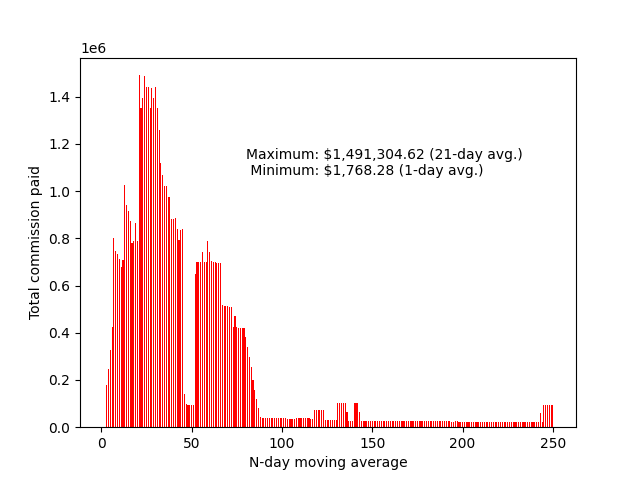
\includegraphics[totalheight=8cm]{figures/total.png}
    \centering
    \caption{Plot of 250 different moving average window sizes and their total profits.}
    \label{total}
\end{figure}
\subsection{Number of Trades Executed}
By varying the size of the moving average window, we also want to see how this affects how many trades will be placed over the time period.
First let's see how window size changes how many times we will buy and sell bitcoin, respectively.

\begin{figure}[h!]
    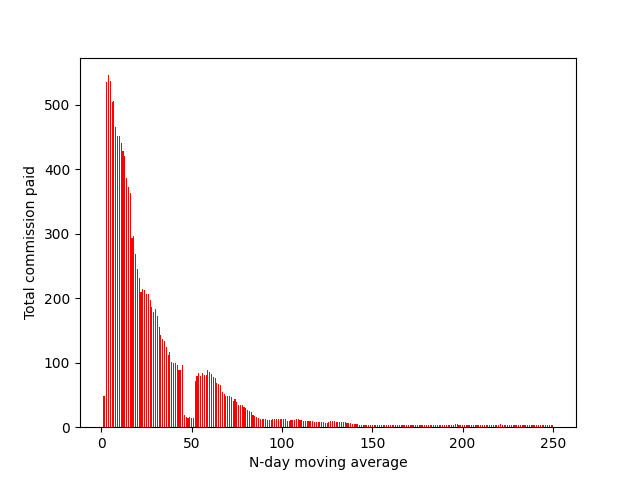
\includegraphics[totalheight=8cm]{figures/btc_pur.png}
    \centering
    \caption{Plot of 250 moving average window sizes and their effect on how many times bitcoin is bought.}
    \label{btc_pur}
\end{figure}


\begin{figure}[h!]
    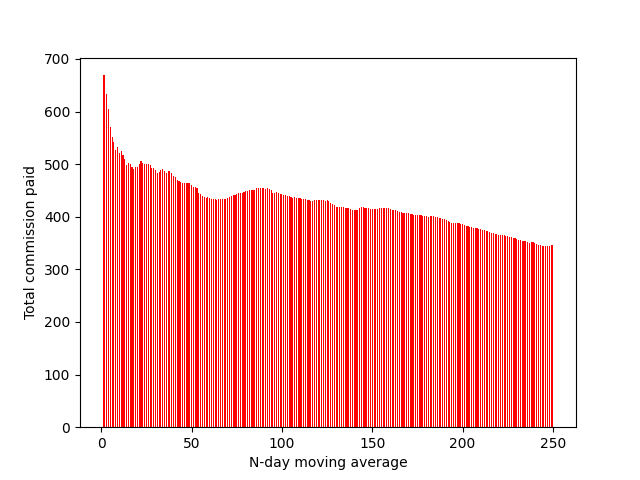
\includegraphics[totalheight=8cm]{figures/btc_sales.png}
    \centering
    \caption{Plot of 250 moving average window sizes and their effect on how many times bitcoin is sold.}
    \label{btc_sales}
\end{figure}
\break
Now let's see the same for gold.
\begin{figure}[h!]
    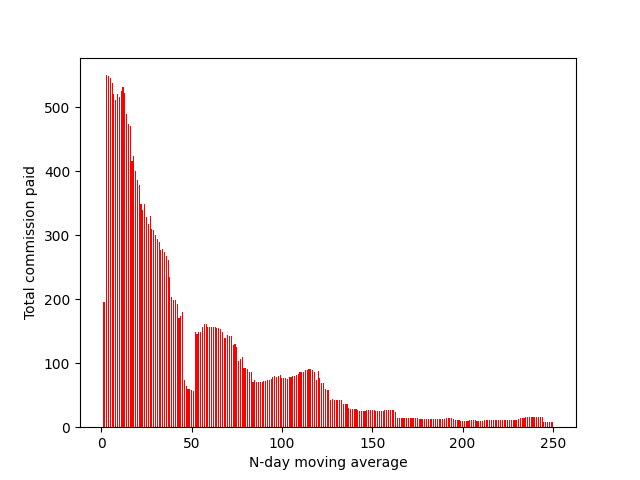
\includegraphics[totalheight=8cm]{figures/gold_pur.png}
    \centering
    \caption{Plot of 250 moving average window sizes and their effect on how many times gold is bought.}
    \label{gold_pur}
\end{figure}

\begin{figure}[h!]
    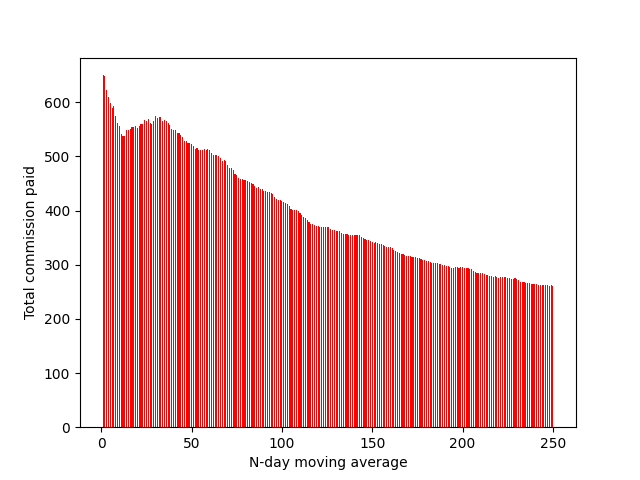
\includegraphics[totalheight=8cm]{figures/gold_sales.png}
    \centering
    \caption{Plot of 250 moving average window sizes and their effect on how many times gold is sold.}
    \label{gold_sales}
\end{figure}

\subsection{Total Commission Paid}
Let's also see how the moving average window size affects how much commission we pay. These commissions eat into total profits, so we want to minimize them. This means minimizing
trading churn, i.e. we only want to trade when we know it is worthwhile to do so to not incur excessive commission penalties.

\begin{figure}[h!]
    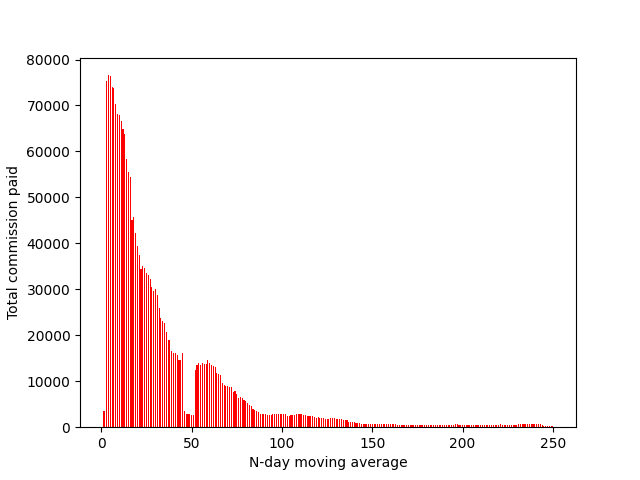
\includegraphics[totalheight=8cm]{figures/comissions.png}
    \centering
    \caption{Plot of 250 moving average window sizes and their effect on total commission paid.}
    \label{commission}
\end{figure}

\section{Analysis}

\subsection{Total Portfolio Value}
As seen in Fig.\ (\ref{total}), it is apparent that the most successful moving average window is 21 days wide. 
There is some interesting behavior around the 50-day window mark where profits drop drastically. It's possible that this is some kind of bug in the model.
Further, max profits for window sizes between 75 to 250 are fairly similar with occasional breakouts at the 120, 135, 140, and 245-day marks.
The results, to some degree, are intuitive: we can't use too small a moving average, otherwise past data isn't taken into consideration, and we can't use too large a 
window otherwise the model will be using overly stale data that is no longer relevant. Thus, with the default parameters given in the problem statement, a 21-day moving average
is ideal for maximum profits.

\subsection{Trading Frequency}
The results in Figs.\ (\ref{btc_pur}), (\ref{btc_sales}), (\ref{gold_pur}), and (\ref{gold_sales}) suggest that larger moving average windows
result in fewer trades made. This makes sense intuitively, since larger windows mean an overly "smooth" moving average where the model will rarely decide to trade assets.
An interesting observation is that the frequency of purchases drops off much more as the window widens compared to sales. This may be due to the fact that both assets over the course
of the five-year period trend upward, meaning it is better overall to buy and hold when possible/ideal and avoid selling too much.

\subsection{Commission}
Because trading frequency decreases for both purchases and sales as the window size increases, it makes sense that total commission decreases consistently as window size increases.
Interestingly, the 21-day moving average window size has some of the highest total commission paid among all window sizes tested, and yet it is still the best size for overall profit.

\section{Possible Improvements}
Immediately, one possible improvement is to take into account the trading restrictions of gold
and unshackle them from trading bitcoin. The higher volatility of bitcoin may allow for some more 
profit. Another improvement would be to implement a system for dynamically adjusting purchase and sale 
quantities, perhaps by assigning a normalized score to each potential trade of how "good" it is and 
increasing or decreasing purchase/sell quantity accordingly. We can also consider using an
exponential moving average instead of a simple one, which assigns weights to previous data depending
on how "recent" it is. Exponential moving averages are calculated as

\begin{equation}
    e_k = \left(p_k \cdot \left( \frac{2}{1+k} \right)\right) + e_{k-1} \cdot \left(1-\left(\frac{2}{1+k}\right)\right)
\end{equation}
where the average is calculated on the $k$-th day and $e_0 = p_0$. The $2$ in this formula is a smoothing factor and can be varied, though $2$ is the most common value used in the real world.
It is possible that this type of moving average is better suited for this problem, though it undoubtedly
requires more computational resources due to its more complex equation and use of recursion. Finally, 
we could add functionality to the model that determines if a trade's potential profit is less than the
potential commission penalty, ensuring we don't make trades that appear to make money but actually result in net losses.


\section{Conclusion}
The best overall moving average window size is 21 days. There is some strange behavior around the 50-day moving average window, seeing as there is a significant drop in both total profit and commission paid.
Though there are a number of improvements we can make to the model for more realistic trading behavior
and possibly even more profits, this current model is a good start, generating \$$1,491,304.62$ in profits over five years, much better than simply purchasing
\$1000 of bitcoin at the start and letting it ride for five years (only about \$45,000 in profits).
\section{References}
1. pandas.DataFrame.ewm — pandas 2.0.3 documentation. (n.d.). Pandas.pydata.org.
\\ https://pandas.pydata.org/docs/reference/api/pandas.DataFrame.ewm.html
\\\\
2.
(2024). Steema.com. \\ https://www.steema.com/docs/financialFunctionsRef/expMovingAverageFunction.htm
%%%%%%%%%%%%%%%%%%%%%%%%%%%%%%
\end{document}
\end